\scanpage{93}
(\uline{PS}) Considérons un arc-demi-cercle $a$
sur $\widetilde D$ ($D$ une p.r. \uline{de ps. droite})
Alors \deleted{$\unsure{a}$}\inserted{$\mathring a$} contient un arc de transition
(ordinaire), sauf dans les \inserted{deux} cas suivants :
\margin{i.e. $a$ contient un arc de transition qui n'a pas d'extrémité en commun avec $a$.}

1°) \deleted{\unsure{Les e.}} Les extrémités $s,s'$ de $a$ \deleted{\unsure{font}} sont élts
d'arcs de généralisation \inserted{$\alpha,\alpha'$} (\unsure{néc. élts de gén.})
[i.e. le pt $\unsure{v}$ de $X$ défini par $(s,s')$ est
un sommet de $X_1$] et il y a une
composante $D_i$ de $X_1$ passant par $v$,
et une orientation $\omega$ de $X$ en $v$, tels
que $D$ soit \deleted{déduit de} ``voisin de $D_i$''
et ``déduit de $D_i$ par petite rotation,
\unsure{autour} $v$'' ; $a\setminus(\mathring\alpha\cap a)\setminus(\mathring\alpha'\cap a)$
est la rive de balayage de $D$
correspondante : $(D_i,v,\omega)$.
\margin{Cas $v\in X_0$}
\margin{\unsure{NB}}
\figure{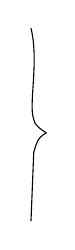
\begin{tikzpicture}[x=.35cm,y=.35cm]
\draw (0,7) .. controls (.3,5.8) and (-.1,4.2) .. (.1,3.7) .. controls (.15,3.4) and (.45,3.3) .. (.55,3.2) .. controls (.2,3) and (.2,2.8) .. (.1,2.5) -- (0,0);
\end{tikzpicture}}

2°) \deleted{Une des deux} \deleted{Les} extrémités $s,s'$ de $a$,
\deleted{\unsure{sont les}} \deleted{\unsure{élts de}} \inserted{extrémités d'}\deleted{\unsure{élts}} \deleted{\unsure{d'un}} arcs de spécialisation
$\alpha_s$, \deleted{$\unsure{\beta}$}$\alpha_{s'}$ (néc. antipodaux l'un
de l'autre !) \inserted{contenus dans $a$} \deleted{alors il existe $p,p'$}
Soit \deleted{$\unsure{\beta}$}\inserted{$\beta$}\unsure{l'arête} de $X_1$ passant par $v$, \deleted{\unsure{et}} et $D_i$
la comp. de $X_1$ contenant $\beta$, il existe
une orientation de $X$ en $\beta$ telle que
$D_i$ \unsure{déduits} —
\margin{Cas $v\notin X_0$}
\figure{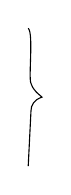
\begin{tikzpicture}[x=.35cm,y=.35cm]
\draw (0,5) .. controls (.2,4.8) and (0,3.2) .. (.1,3) .. controls (.2,2.7) and (.4,2.6) .. (.5,2.5) .. controls (.2,2.4) and (.1,2.2) .. (.1,2) -- (0,0);
\end{tikzpicture}}
\margin{\uline{NB} Dans ce cas, $a$ contient deux arcs de spécialisation,
\deleted{\unsure{de gén.}} (mais à \unsure{un côté} en commun)}

\margin{\uline{NB} Dans le cas des ps. droites, si \unsure{on a}
sur $\widetilde D$ une transition (avec \unsure{sa rive de contrebal.} en pointillés)
\figure{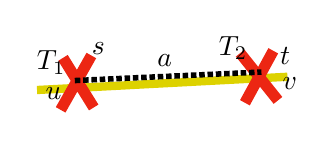
\begin{tikzpicture}[x=.6cm,y=.6cm]
\draw[yellow!70!olive,line width=3pt] (-.8,-.08)--(4.5,.2);
\draw[red!70!brown,line width=4pt] (-.3,-.5)--(.35,.65) (-.25,.6)--(.4,-.45) (3.6,-.35)--(4.2,.75) (3.5,.7)--(4.3,-.3);
\draw[black,densely dotted,line width=2pt] (0,.12)--(3.95,.3);
\node at (1.9,.55) {$a$};\node at (-.5,.5) {$\unsure{T_1}$};\node at (3.35,.8) {$\unsure{T_2}$};
\node at (.5,.8) {$s$};\node at (4.45,.65) {$t$};\node at (-.45,-.15) {$u$};\node at (4.55,.05) {$v$};
\end{tikzpicture}}
les conditions suivantes sont \inserted{équivalentes} :
a) $s,t$ \unsure{non-alignés},
b) $u\ne v'$ (\unsure{antip. de $v$})
c) dist. comb. de $u$ à $v$ est \inserted{(sur $\unsure{\widetilde D}$)} \deleted{$\unsure{\le n}$}\inserted{$\le n-1$},
d) après spécialisation \unsure{(de $T_1$)}, \unsure{en un point spécifique}, \unsure{vis. $T_2$} ($\unsure{\Leftrightarrow s=t}$)
}
\margin{\deleted{\unsure{dans le} \unsure{deux cas} \unsure{$v$ et $v'$} \unsure{sont l'unique} \unsure{comp. incid. de}}}
\figure{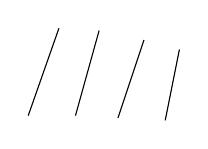
\begin{tikzpicture}[x=.3cm,y=.3cm]\draw (0,0)--(1.3,3.7) (2,0)--(3,3.6) (3.8,-.1)--(4.9,3.2) (5.8,-.2)--(6.4,2.8);\end{tikzpicture}}

C'est cette circonstance qui
suggère qu'il n'y a que
deux sortes de sommets
dans $\mathcal X$, les sommets
d'ordre 4 dont je viens de
parler, et les sommets
correspondant aux \unsure{systèmes}
$(D_i,\beta,\omega)$, où \deleted{$\unsure{\beta}$}$D_i$ est une
``composante irr. de $X_1$'' qui est un
cercle topologique dans $X$, $\beta$ une
facette de $D_i$ (sommet ou arête)
$\omega$ une orientation de $X$ en $\beta$.
Sinon, on n'a pas de contrôle, a
priori, sur le type des ``circuits-
sommets'' sur $\mathcal X$ — et \unsure{j'ajoute}
qu'il n'est pas clair \deleted{\unsure{en quoi}} dans
quelle mesure le transport
parallèle sur les $\mathrm{Pol}(D)$ \unsure{passe}
en un syst. local sur $\mathcal X$.
\margin{92}
